\documentclass[11pt,reqno,twoside]{article}
%>>>>>>> RENAME CURRENT FILE TO MATCH LECTURE NUMBER
% E.g., "lecture_01.tex"

%>>>>>>> DO NOT EDIT MACRO FILE

% >>>> DO NOT EDIT THIS FILE
% If you *must* add or change a macro, please email fkoh@caltech.edu

%=================================================
% Basics
%=================================================

\usepackage{fixltx2e} % Makes \( \) equation style robust, among other
                      % things. Must be the first package.


% Makes ligatured fonts searchable and copyable in pdf readers
\usepackage{cmap} % Load before fontenc 

% Always include these font encodings in your document 
% unless you have a very good reason.
\usepackage[T1]{fontenc}
\usepackage[utf8]{inputenc}

\usepackage{verbatim}

%=====================================
% Look & feel
%=====================================

% Allows for manual space setting
\usepackage{setspace}

%=============
% Fonts
%=============

\usepackage{lmodern} % Improved version of computer modern
\usepackage[scale=0.88]{tgheros} % Helvetica clone for sans serif font


\newcommand\hmmax{2} % Default is 3.
\newcommand\bmmax{2} % Default is 4.

\usepackage{bm} % boldmath must be called after the package
\providecommand{\mathbold}[1]{\bm{#1}}

%=============
% AMS Packages and fonts
%=============
\usepackage{amsmath,amsbsy,amsgen,amscd,amsthm,amsfonts,amssymb} 

%=============
% Margins and paper size
%=============
\usepackage[centering,top=1.5in,bottom=1.2in,left=1.4in,right=1.4in]{geometry}

%=============
% Title setup
%=============
\usepackage{titling}
%\usepackage{nopageno}
\setlength{\droptitle}{-7.5em}

\pretitle{\noindent\rule{0.85\linewidth}{0.2mm}\par%
  \begin{raggedright}\LARGE\sffamily}
\posttitle{\par\end{raggedright}%
\noindent%
\rule{0.85\linewidth}{0.5mm}\par}

\preauthor{\noindent\vspace{0.5em}%
  \sffamily\begin{tabular}[t]{ll}}
  \postauthor{\end{tabular}\par\thispagestyle{plain}}

\predate{\noindent%
  \small\sffamily\itshape\begin{tabular}[t]{l}%
    ACM 256, Winter 2019 \\ %
    Dr.\ Franca Hoffmann \\ %
  }
  \postdate{
  \end{tabular}\par}

%=============
% Section headings
%=============
\usepackage[sf,bf,compact]{titlesec}

%=============
% Tables and lists
%=============
\usepackage{booktabs,longtable,tabu} % Nice tables
\setlength{\tabulinesep}{1mm}
\usepackage[font=small,margin=10pt,labelfont={sf,bf},labelsep={space}]{caption}


\usepackage{enumitem}
\setitemize{itemsep=0pt} 
\setenumerate{itemsep=0pt}
\setlist{labelindent=\parindent,%  % Recommended by enumitem package
  font=\sffamily}


%=============
% Hyperlink colors
%=============
\usepackage[usenames,dvipsnames]{xcolor}
\definecolor{dark-gray}{gray}{0.3}
\definecolor{dkgray}{rgb}{.4,.4,.4}
\definecolor{dkblue}{rgb}{0,0,.5}
\definecolor{medblue}{rgb}{0,0,.75}
\definecolor{rust}{rgb}{0.5,0.1,0.1}

\usepackage{url}
\usepackage[colorlinks=true]{hyperref}
\hypersetup{linkcolor=dkblue}    
\hypersetup{citecolor=rust}      
\hypersetup{urlcolor=rust}     

%=============
% Microtype
%=============
\usepackage[final]{microtype} 

%=============
% Theorems, etc.
%=============
\newtheoremstyle{myThm} % name
    {\topsep}                    % Space above
    {\topsep}                    % Space below
    {\itshape}                   % Body font
    {}                           % Indent amount
    {\sffamily\bfseries}                   % Theorem head font
    {.}                          % Punctuation after theorem head
    {.5em}                       % Space after theorem head
    {}  % Theorem head spec (can be left empty, meaning ‘normal’)

\newtheoremstyle{myRem} % name
    {\topsep}                    % Space above
    {\topsep}                    % Space below
    {}                   % Body font
    {}                           % Indent amount
    {\sffamily}                   % Theorem head font
    {.}                          % Punctuation after theorem head
    {.5em}                       % Space after theorem head
    {}  % Theorem head spec (can be left empty, meaning ‘normal’)

\newtheoremstyle{myDef} % name
    {\topsep}                    % Space above
    {\topsep}                    % Space below
    {}                   % Body font
    {}                           % Indent amount
    {\sffamily\bfseries}                   % Theorem head font
    {.}                          % Punctuation after theorem head
    {.5em}                       % Space after theorem head
    {}  % Theorem head spec (can be left empty, meaning ‘normal’)

\theoremstyle{myThm}
\newtheorem{theorem}{Theorem}[section]
\newtheorem{lemma}[theorem]{Lemma}
\newtheorem{proposition}[theorem]{Proposition}
\newtheorem{corollary}[theorem]{Corollary}
\newtheorem{fact}[theorem]{Fact}

\theoremstyle{myRem}
\newtheorem{remark}[theorem]{Remark}

\theoremstyle{myDef}
\newtheorem{definition}[theorem]{Definition}
\newtheorem{example}[theorem]{Example}

%=====================
% Header
%=====================
\usepackage{fancyhdr}
\usepackage{nopageno} % Gets rid of page number at the bottom
\fancyhf{} % Clear header style
\renewcommand{\headrulewidth}{0.5pt} % remove the header rule
\pagestyle{fancy}
\fancyhead[LE,RO]{\textsf{\small \thepage}}

\setlength{\headheight}{14pt}
%=====================
% Fix delimiters
%=====================

% Fixes \left and \right spacing issues. See discussion at
% http://tex.stackexchange.com/questions/2607/spacing-around-left-and-right
\let\originalleft\left
\let\originalright\right
\renewcommand{\left}{\mathopen{}\mathclose\bgroup\originalleft}
\renewcommand{\right}{\aftergroup\egroup\originalright}

%=================================================
% Math macros
%=================================================

%=============
% Generalities
%=============
\usepackage{mathtools}
\mathtoolsset{centercolon}  % Makes := typeset correctly for definitions

%%% Equation numbering
%\numberwithin{equation}{section} 

%%% Annotations
\newcommand{\notate}[1]{\textcolor{red}{\textbf{[#1]}}}

%==============
% Symbols
%==============
\let\oldphi\phi
\let\oldeps\epsilon
\let\oldemptyset\emptyset
\let\emptyset\varnothing

\renewcommand{\phi}{\varphi}
\renewcommand{\epsilon}{\varepsilon}
\newcommand{\eps}{\varepsilon}
\newcommand{\cl}{\mathrm{cl}}
\newcommand{\wto}{\rightharpoonup}
\newcommand{\wsto}{\overset{\ast}{\rightharpoonup}}
\newcommand{\wwto}{\overset{w}{\to}}
\newcommand{\wwsto}{\overset{w*}{\to}}

%==============
% Constants
%==============

% Set constants upright
\newcommand{\cnst}[1]{\mathrm{#1}}  
\newcommand{\econst}{\mathrm{e}}
\newcommand{\rd}{\mathrm{d}}
\newcommand{\dist}{\mathrm{dist}}

\newcommand{\zerovct}{\vct{0}} % Zero vector
\newcommand{\Id}{\mathbf{I}} % Identity matrix
\newcommand{\onemtx}{\bm{1}}
\newcommand{\zeromtx}{\bm{0}}

%==============
% Sets
%==============
\providecommand{\mathbbm}{\mathbb} % In case we don't load bbm

% Reals, complex, naturals, integers, field
\newcommand{\R}{\mathbbm{R}}
\newcommand{\C}{\mathbbm{C}}
\newcommand{\N}{\mathbbm{N}}
\newcommand{\Z}{\mathbbm{Z}}
\newcommand{\F}{\mathbbm{F}}

%==============
% Probability
%==============
\newcommand{\Prob}{\operatorname{\mathbbm{P}}}
\newcommand{\Expect}{\operatorname{\mathbb{E}}}

%==============
% Vectors and matrices 
%==============
\newcommand{\vct}[1]{\mathbold{#1}}
\newcommand{\mtx}[1]{\mathbold{#1}}

%=============
% Operators
%=============
\newcommand{\B}{\mathcal{B}}
\newcommand{\op}[1]{\mathbold{#1}}

 % "macro.tex" must be in the same folder

%>>>>>>> IF NEEDED, ADD A NEW FILE WITH YOUR OWN MACROS

% \input{lecture_01_macro.tex} % Name of supplemental macros should match lecture number

%>>>>>>> LECTURE NUMBER AND TITLE
\title{Clase 0:               % UPDATE LECTURE NUMBER
    Aprendizaje Estadístico}	% UPDATE TITLE
% TIP:  Use "\\" to break the title into more than one line.

%>>>>>>> DATE OF LECTURE
\date{Enero 14, 2021} % Hard-code lecture date. Don't use "\today"

%>>>>>>> NAME OF SCRIBE(S)
\author{%
  Responsable:&
  Mr Bean  % >>>>> SCRIBE NAME(S)
}

\begin{document}
\maketitle %  LEAVE HERE
% The command above causes the title to be displayed.

%>>>>> DELETE ALL CONTENT UNTIL "\end{document}"
% This is the body of your document.

\section{Introducción}
\label{sec:introduction}

La idea de este documento es proporcionar una guía para escribir las notas de la
clase. Recuerda todos en la clase usarán las notas así que que cuida que sean
claras y concisas. A continuación, se encuentran algunas reglas diseñadas para
garantizar la coherencia en las notas del curso, así como algunos consejos para
aprovechar al máximo este archivo.

\subsection{Básicos}

Para componer este archivo, necesitas tener una copia razonablemente actualizada
de \LaTeX\ instalada en tu computadora. Este software es gratuito y está
disponible en \url{http://tug.org}. Consulte la Sección~\ref{sec:need-help}
para obtener información sobre dónde obtener más ayuda para configurar \LaTeX,
componer matemáticas y otros problemas técnicos.

Para comenzar, descargue y extraiga el archivo \texttt{notas-template.zip} del
repositorio del curso. Esta carpeta comprimida contiene los siguientes archivos.
\begin{description}
  \setlength{\itemsep}{0pt} \setlength{\topsep}{0pt} % Make list compact
\item[\texttt{template.pdf}] \emph{Este documento.}
\item[\texttt{template.tex}] \emph{Contiene el código fuente de este documento.} Los comentarios indican los cambios que se deben realizar para iniciar. Por ejemplo, debes agregar el número y el título de la clase, incluir tu nombre y la fecha de la clase que estás transcribiendo.
\item[\texttt{template.bib}] \emph{Archivo con las referencia en formato BibTeX.}
\item[\texttt{macro.tex}] \emph{Define el estilo y los shortcuts.}
\item[\texttt{bell\_curve\_hand.jpg}, \texttt{bell\_curve\_matlab.pdf}]  \emph{Las imágenes \Cref{fig:bell-curve}.}
\end{description}
Para compilar desde una terminal utiliza los comandos
\begin{center}
  \begin{minipage}[c]{0.3\linewidth}
\begin{verbatim}
 pdflatex template.tex
 bibtex template
 pdflatex template.tex
 pdflatex template.tex
\end{verbatim}
  \end{minipage}
\end{center}

\subsection{Configurando tus notas de clase}
\label{sec:setting-up-your}

Cambia el nombre de todos los archivos \texttt{template.*} a
\texttt{lecture\_XX.*}, donde \texttt{XX} es el número de la clase. Por ejemplo,
el archivo fuente de la primera se llamará \texttt{lecture\_01.tex}. Si se
necesitan incluir referencias, incluye las entradas BibTeX con el formato
apropiado en su archivo \texttt{lecture\_XX.bib}.

\section{Reglas}
\label{sec:rules}
Para que las notas sean lo más coherentes posible, vamos a hacer cumplir algunas reglas básicas. Estas reglas están pensadas como guías, sin embargo cuando el sentido común y las reglas entren en conflicto, le daremos preferencia al primero.

\subsection{Estilo}
\label{sec:style}

El contenido es la parte mas importante de las notas. Sin embargo, es importante mantener consitstencia en la notación.

\begin{description}\setlength{\itemsep}{0pt} % Compact description list
\item[Idioma] Utiliza oraciones en español completas y gramaticalmente correctas. Consulta diccionarios y guías de estilo para conocer la ortografía y uso adecuados. Para obtener pautas específicas sobre escritura matemática, consulta~\cite{Che:,Hal:70,Hig:98}.
\item[Secciones] Usa los comandos de  \LaTeX para definir secciones, subsecciones, subsubsecciones, etc.  Trata de utilizar la numeración y títulos que seguimos en clase para las secciones. Para secciones adicionales por favor utiliza el sentido común.
\item[Ecuaciones] Las ecuaciones sólo se enumerarán cuando son referenciadas en el texto. Consulta la guía de Michael Downes \href{https://math.mit.edu/~dav/short-math-guide.pdf}{Short Math Guide for \LaTeX} para tener una idea de los ambientes de ecuaciones.
\item[Teoremas, definiciones, etc.] Hay distintos ambientes para escribir resultados formales. Por ejemplo, el ambiente de teoremas, \texttt{theorem}, se utiliza como:
  \begin{center}
    \begin{minipage}[c]{0.7\linewidth}
      \begin{theorem}[Fermat, Wiles]\label{thm:FermatWiles}
        Para cualquier $n \ge 3$, y cualquier $a,b,c \in \N,$ se tiene que
        $a^n + b^n \ne c^n.$
      \end{theorem}
      \begin{proof}
        Bastante larga para estas notas.
      \end{proof}
    \end{minipage}
  \end{center}
  Ejemplos de otros ambientes son \texttt{lemma}, \texttt{proposition}, \texttt{corollary}, \texttt{fact}, \texttt{remark}, \texttt{definition}, y \texttt{example}.
\item[Figuras] Por favor incluye figuras cuando sea apropiado. Imágenes escaneadas son aceptables siempre y cuando sean legibles, pero también no duddes en incorporar figuras hechas con software. Todas las figuras deben de tener leyendas adecuadas. El compilar \texttt{pdflatex} sólo acepta figuras en formato \texttt{.pdf} (para imágenes por vectores), \texttt{.png} (diagramas simples y figuras rasterizadas), o \texttt{.jpg} (para fotos). Ve la \cref{fig:bell-curve} como ejemplo.
    \begin{figure}[h!]
      \centering
      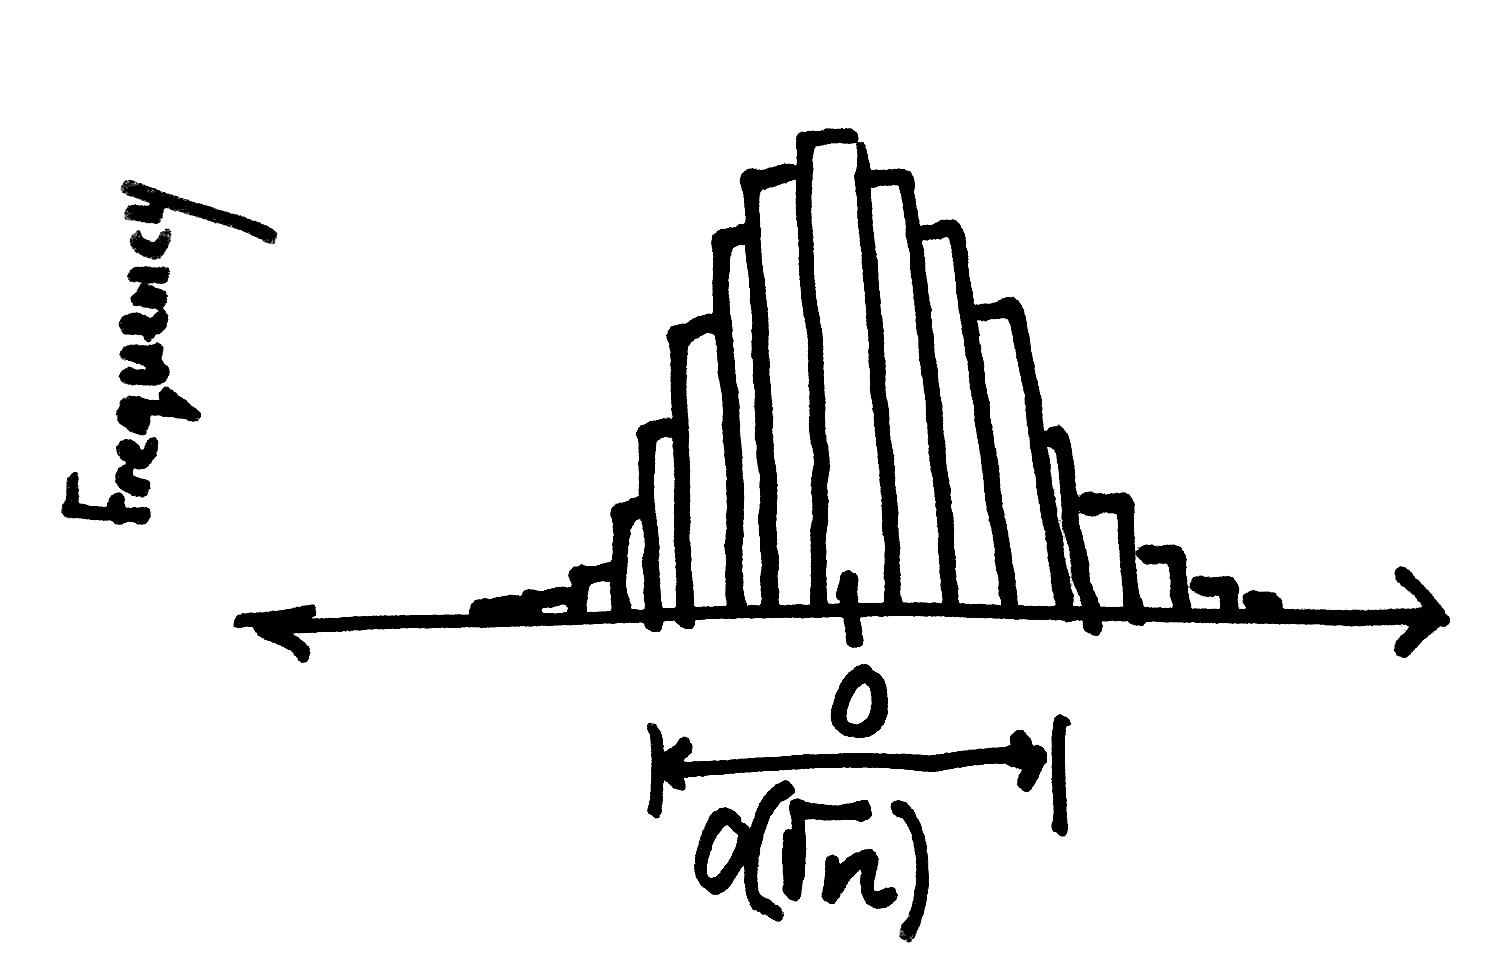
\includegraphics[width=0.4\columnwidth]{bell_curve_hand.jpg}
      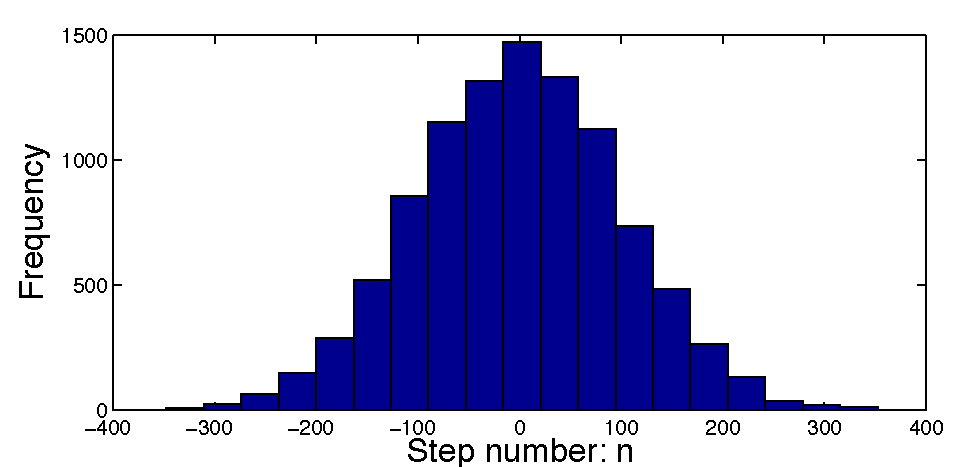
\includegraphics[width=0.55\columnwidth]{bell_curve_matlab.pdf}
      \caption{{\textsf{Figuras de ejemplo.}}  Figuras hechas a mano [izquierda] son aceptables para las notas, pero asegurate de quitar cualquier espacio muerto alrededor.   Si prefieres usar algún software para generar las imágenes [derecha] cuida que los ejes y las anotaciones sean suficientemente grandes}\label{fig:bell-curve}
    \end{figure}

\item[Márgenes] No dejes que los ecuaciones o el texto invada el margen a la derecha.  \LaTeX\ muchas veces es suficiente para manejar este detalle, pero habrá situaciones en las que tendrás que parafrasear para evitar esta invasión. Las ecuaciones requirirán de mayor trabajo. Si una ecuación es muy larga usa los ambientes \texttt{multline} o \texttt{align} para ajustar al tamaño de línea.
\item[Puntuación] Un documento matemático también reglas de puntuación usuales. Esto incluye commas y puntos despues de escribir una ecuación o expresiones matemáticas. Un buen principio es colocar la puntuación donde lo esperarías si las matemáticas que escribes se leyeran como palabras. Si una coma/punto está al final de una ecuación (por ejemplo, en entornos \texttt{equation}, \texttt{align} o \texttt{multiline}), está precedido por \verb|\,| para crear un espacio pequeño. Por ejemplo, la ecuación $ a ^ n + b ^ n \ne c ^ n $ del \cref{thm:FermatWiles} en una línea separada debe mostrarse como
  \begin{equation}
      a^n + b^n \ne c^n \,.
  \end{equation}
\item[Notación] Mantén la notación que usemos en clase. Por consistencia, considera la notación siguiente

    \begin{minipage}[c]{\linewidth}
      \begin{center}
        \begin{tabu}{ccc}
          \toprule
          \textbf{Propósito} &  \textbf{Ejemplo} \\
          \midrule
          Naturales, enteros  & $\N$, $\Z$
          \\
          Reales, complejos  & $\R$, $\C$
          \\
          Campos (reales o complejos) & $\F$
          \\
          Normas & $\| \cdot \|$
          \\
          Producto interior & $ \langle \cdot, \cdot \rangle$
          \\
          Valores esperados & $\Expect_{z \sim \D}[f(z)]$
          \\
          Límites & $\underset{\theta \in \Theta}{\sup} \,\, \mathcal{L}_n(\theta)$
          \\
          \bottomrule
        \end{tabu}
      \end{center}
    \end{minipage}

    Consulta el archivo fuente \texttt{template.tex} para ver los comandos que se utilizaron para construir esta tabla. Adicionalmente, utiliza el símbolo $\rd$ para las integrales, precedido por \verb|\,| para incorporar un pequeño espacio. Aqui un ejemplo $\int f(x)\, \rd x.$
  \item[Referencias cruzadas ] Usa la funcionalidad de \LaTeX para hacer referencia a secciones, teoremas, tablas, figurass y ecuaciones. Por ejemplo, este texto se encuentra en la Seccion~\ref{sec:style}, que empieza en la página~\pageref{sec:style}. Escribir los números hace tu documento frágil y susceptible a mucho trabajo adicional. De igual forma, no puedes incluir ligas útiles como las que provee el paquete \texttt{hyperref}.
  \item[Bibliografía] Si necesitas citar un trabajo, utiliza \texttt{bibtex} con estilo \texttt{siam}. Las entradas se necesitan llenar de acuerdo al formato  AMS, incluyendo \href{http://www.ams.org/msnhtml/serials.pdf}{las abreviaciones y número de serie} correctos. Para muchos textos publicados puedes descargar el formato \texttt{bibtex} aceptado de la página de la AMS~\cite{mathscinet}. Por favor, incluye las referencias BibTeX en un archivo con nombre \texttt{lecture\_XX.bib}.

\end{description}

\subsection{Edición}
\label{sec:editing}

Ningún documento escrito está completo sin una edición completa, y hay varias
herramientas disponibles para ayudarte a editar tus archivos \LaTeX. Una
búsqueda rápida en la web muestra varios correctores ortográficos.
Desafortunadamente, los correctores gramaticales automáticos resultan inútiles
para los documentos matemáticos debido a la gran cantidad de ecuaciones. Por lo
tanto, debes revisar la gramática tú mismo.

Hay varias herramientas útiles disponibles para la edición colaborativa de documentos \LaTeX. Podemos utilizar \texttt{\textbackslash notate} que \notate {resalta el texto en rojo}. Algunas utilidades incluidas en la distribución \TeX\ incluyen \texttt{latexdiff}, que muestra las diferencias entre los archivos \TeX, y \textit{Excalibur}, un corrector ortográfico compatible con \LaTeX.

También podemos hacer uso de la plataforma de Github para hacer las revisiones
necesarias.

\subsection{¿En verdad necesitas atajos?}
\label{sec:macros}

El objetivo es tener un conjunto coherente de notas de clase para el beneficio de todos. En especial, como material de referencia. Idealmente, los compilaremos en un solo documento con una tabla de contenido. Esto será imposible si los escribas cambian las macros.

Es por esto que es importante mantener las macros en \texttt{macro.tex}. Por
favor no las cambies.  No uses el commando \texttt{\textbackslash renewcommand}.
Si te es mas útil tener las propias, por favor incluyelas en un archivo separado
\texttt{lecture\_XX\_macros.tex} donde \texttt{XX} es el número de la clase que
estás transcribiendo.  Asegúrate que no haya porblemas con las preexistentes.


\section{Ayuda}
\label{sec:need-help}

Para obtener información sobre composición usando \LaTeX, se recomienda \href
{https://math.mit.edu/~dav/short-math-guide.pdf}{Short Math Guide for \LaTeX} de
Michael Downes y las referencias que contiene. Numerosos recursos adicionales
para \LaTeX\ están disponibles en internet, incluido el sitio
\href{http://tex.stackexchange.com/}{\TeX\ StackExchange}. Antes de contactar al
profesor trata de resolver tu duda buscando en dichos foros.


Si encuentra un error en la plantilla o en el archivo de macro, envíame un
mensaje por canvas con la descripción del problema y la solución que tengas en
mente.


%>>>>>> END OF YOUR CONTENT

%>>>>>>>>>> take acknowledgements out
\section*{Agradecimientos} Este {\emph template} se ha adaptado y traducido del
provisto en la clase ACM 204 (Otoño 2017) por el profesor Joel Tropp.


\bibliographystyle{siam} % <<< USE "alpha" BIBLIOGRAPHY STYLE
\bibliography{template} % <<< RENAME TO "lecture_XX"


\end{document}
